\subsection{Cuantificación de incertidumbre para imágenes médicas mediante FBPINN}

En esta sección se aborda la cuantificación de la incertidumbre en un conjunto de datos de imágenes de estructuras vasculares (venas). Estas imágenes fueron reconstruidas a través de un modelo de Redes Neuronales Informadas por la Física (PINN); en particular, se empleó la arquitectura de PINN Basada en Bases Finitas (FBPINN).

Como se describió previamente, la aplicación de la predicción conforme requiere definir inicialmente una función de puntuación de no conformidad. Para este propósito, se propone utilizar la norma $\mathbb{L}_1$, definida formalmente como:
\begin{equation}
    S = |y - \hat{y}|
\end{equation}

\begin{figure}[H]
    \centering
    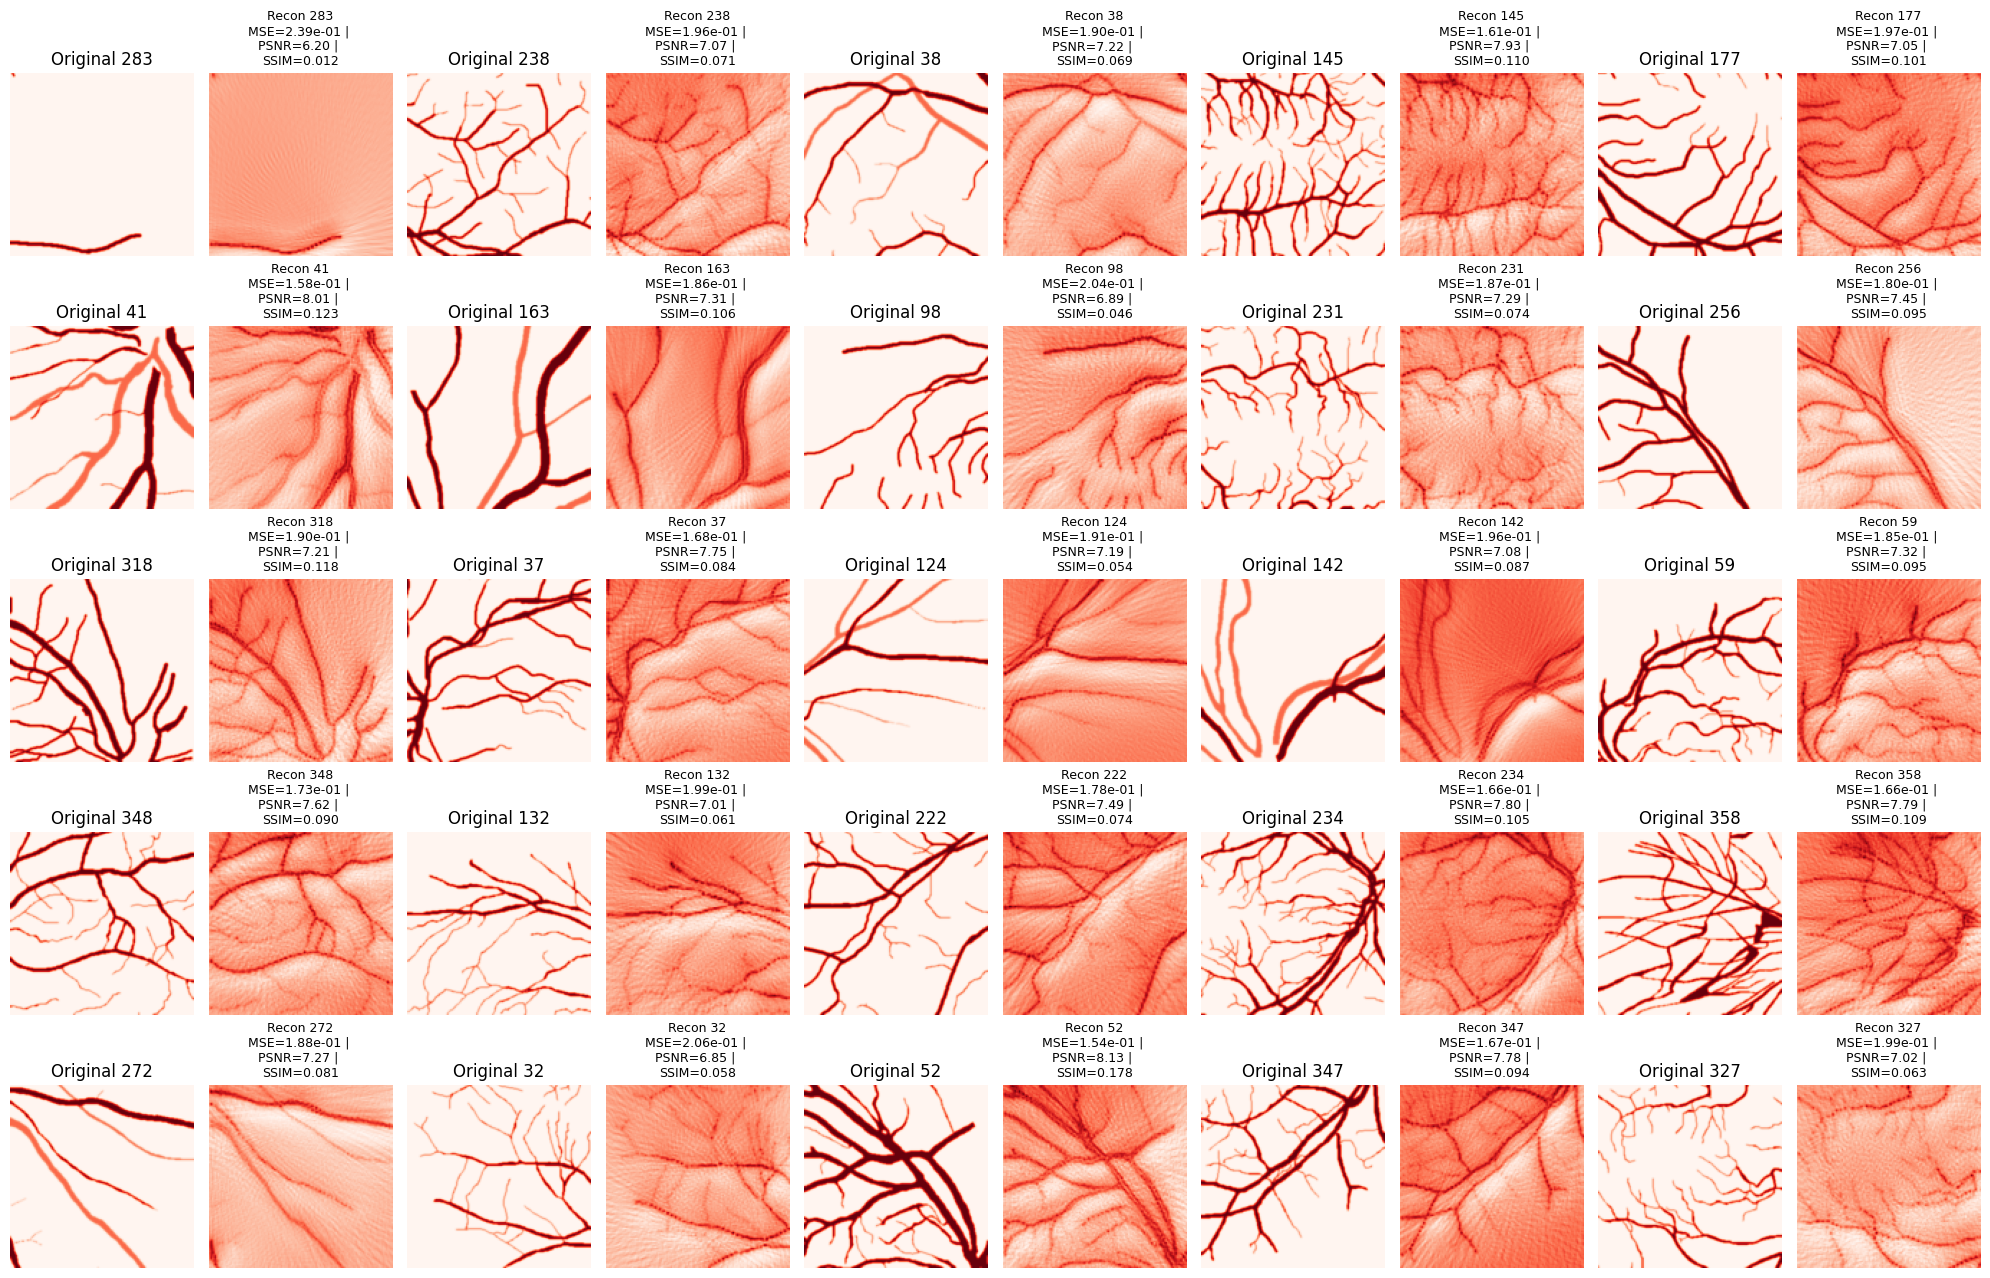
\includegraphics[width=1\linewidth]{img/data_init.png}
    \caption{Imágenes médicas reconstruidas mediante FBPINN y resolución del problema inverso.}
    \label{fig:data_fbpinn}
\end{figure}

Es fundamental destacar que el modelo no toma como entrada la imagen original directamente, sino una reconstrucción fundamentada en funciones gaussianas. El operador aprende a reconstruir la onda acústica a través del pulso gaussiano aplicándolo a cada coordenada espacial de la imagen, generando así un sinograma. Posteriormente, este sinograma es procesado por un algoritmo determinista que resuelve el problema inverso para reconstruir la imagen final.

Por lo tanto, la entrada efectiva al modelo se denota como $y_{\text{reconstruida}} = p_0$, la cual representa una matriz espacial con los valores de presión inicial para cada píxel. Sobre esta base, se procede a aplicar un conjunto de algoritmos de predicción conforme con carácter exploratorio.

\subsubsection{Split Conformal Prediction (SCP) en FBPINN}

En primera instancia, se evalúa el algoritmo SCP aplicado de forma independiente píxel a píxel, modalidad que se denota en la literatura como calibración condicional local. Es imperativo resaltar que el algoritmo SCP convencional ofrece, por definición, una garantía de cobertura marginal; es decir, el nivel de confianza se cumple en el promedio de la imagen y no necesariamente de manera condicional para cada píxel de forma aislada.

Para mitigar la varianza en la estimación de los cuantiles locales y aproximar una cobertura condicional robusta, se requiere disponer de un volumen considerable de muestras en el conjunto de calibración.

\begin{figure}[H]
    \centering
    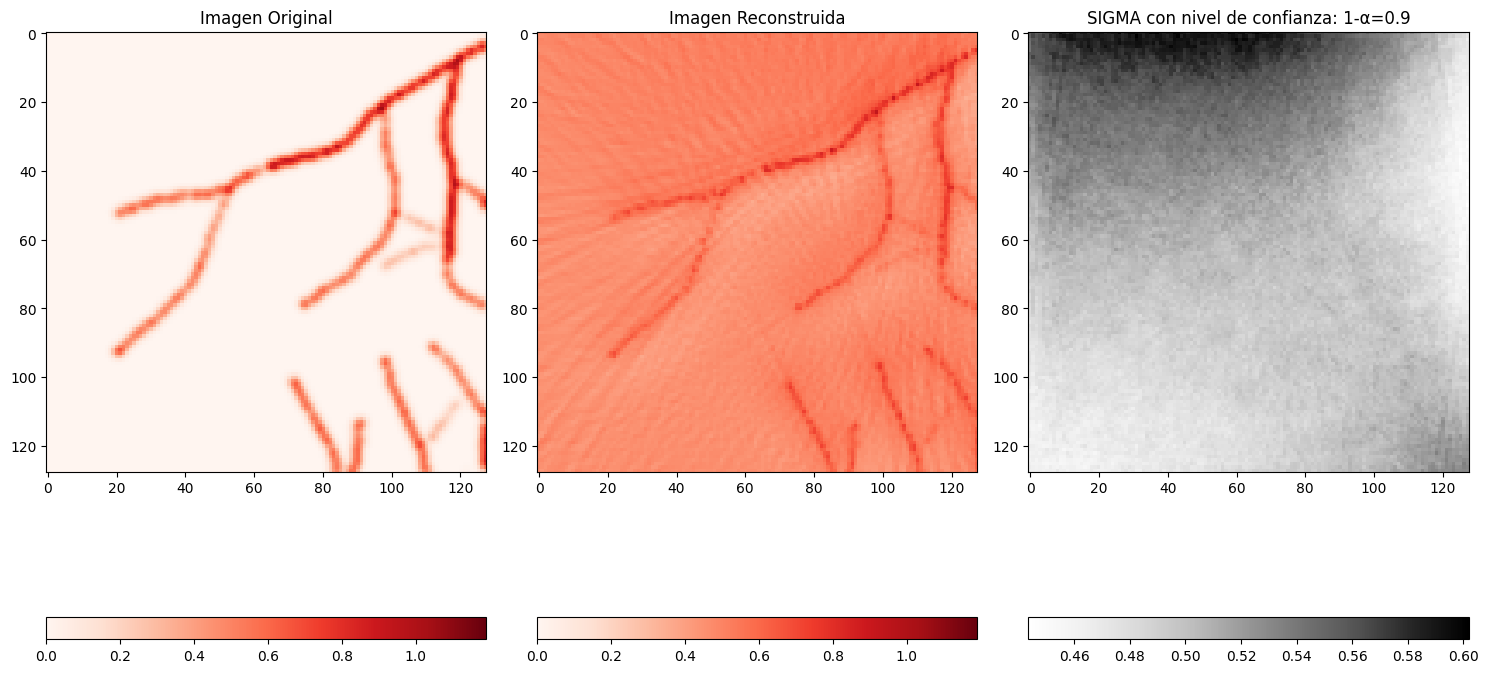
\includegraphics[width=0.8\linewidth]{img/scp_fbpinn.png}
    \caption{Split Conformal Prediction aplicado bajo calibración condicional, donde $\sigma = \hat{q}$.}
    \label{fig:scp_fbpinn}
\end{figure}

Un aspecto analítico relevante observado en la Figura~\ref{fig:scp_fbpinn} es que el umbral $\hat{q}$ deja de ser un escalar constante para todo el dominio. En su lugar, se transforma en una matriz que preserva la dimensión espacial de la imagen, de modo que $\hat{q} \in \mathbb{R}^{H \times W}$.

Esta técnica proporciona una caracterización topográfica general de la incertidumbre a lo largo de la malla de píxeles, permitiendo formular una región de predicción conforme de la forma $\hat{f}(X_{\text{test}}) \pm \hat{q}$. No obstante, estos intervalos de confianza resultan idénticos para cualquier instancia del conjunto de prueba $(\mathcal{X}, \mathcal{Y})_{\frac{n}{2} + 1, \dots, n}$, a pesar de que la física del problema sugiere que la incertidumbre debería exhibir variaciones dinámicas entre imágenes.

Con el objetivo de introducir dependencia de la muestra en la inferencia, e inspirándonos en el método de puntuación por residuo escalado, se propone una modificación adaptativa. Mientras que la etapa de calibración permanece invariante, la incertidumbre resultante para la fase de prueba se escala mediante la siguiente formulación:

\begin{equation}
    \sigma_q = \frac{q(i,j)^{\alpha}}{\mathcal{\hat{\pi}}(y \in \mathcal{R}_1|x)(i,j)}
\end{equation}

Donde el término $\mathcal{\hat{\pi}}(y \in \mathcal{R}_1|x)(i,j)$ representa la probabilidad condicional de que el píxel en la coordenada $(i,j)$ pertenezca a la estructura vascular (vena), $q(i,j)^{\alpha}$ es debido a que por cada $\alpha$ seteado se obtendrá una nueva matriz de $q(i,j)$.

Para estimar esta distribución, la imagen se segmenta mediante el algoritmo de Expectación-Maximización (EM) usando mezcla de gaussiandas  sobre el espacio de intensidades de los píxeles los cuales fueron clusterizados con y sin ecualización previa.

El proceso consiste en normalizar las intensidades del histograma al intervalo $[0, 255]$ para posteriormente ajustar el modelo de mixturas que infiere la probabilidad píxel a píxel. Esta probabilidad actúa como una máscara adaptativa que genera regiones de incertidumbre dinámicas y específicas para cada imagen de prueba.

\begin{figure}[H]
    \centering
    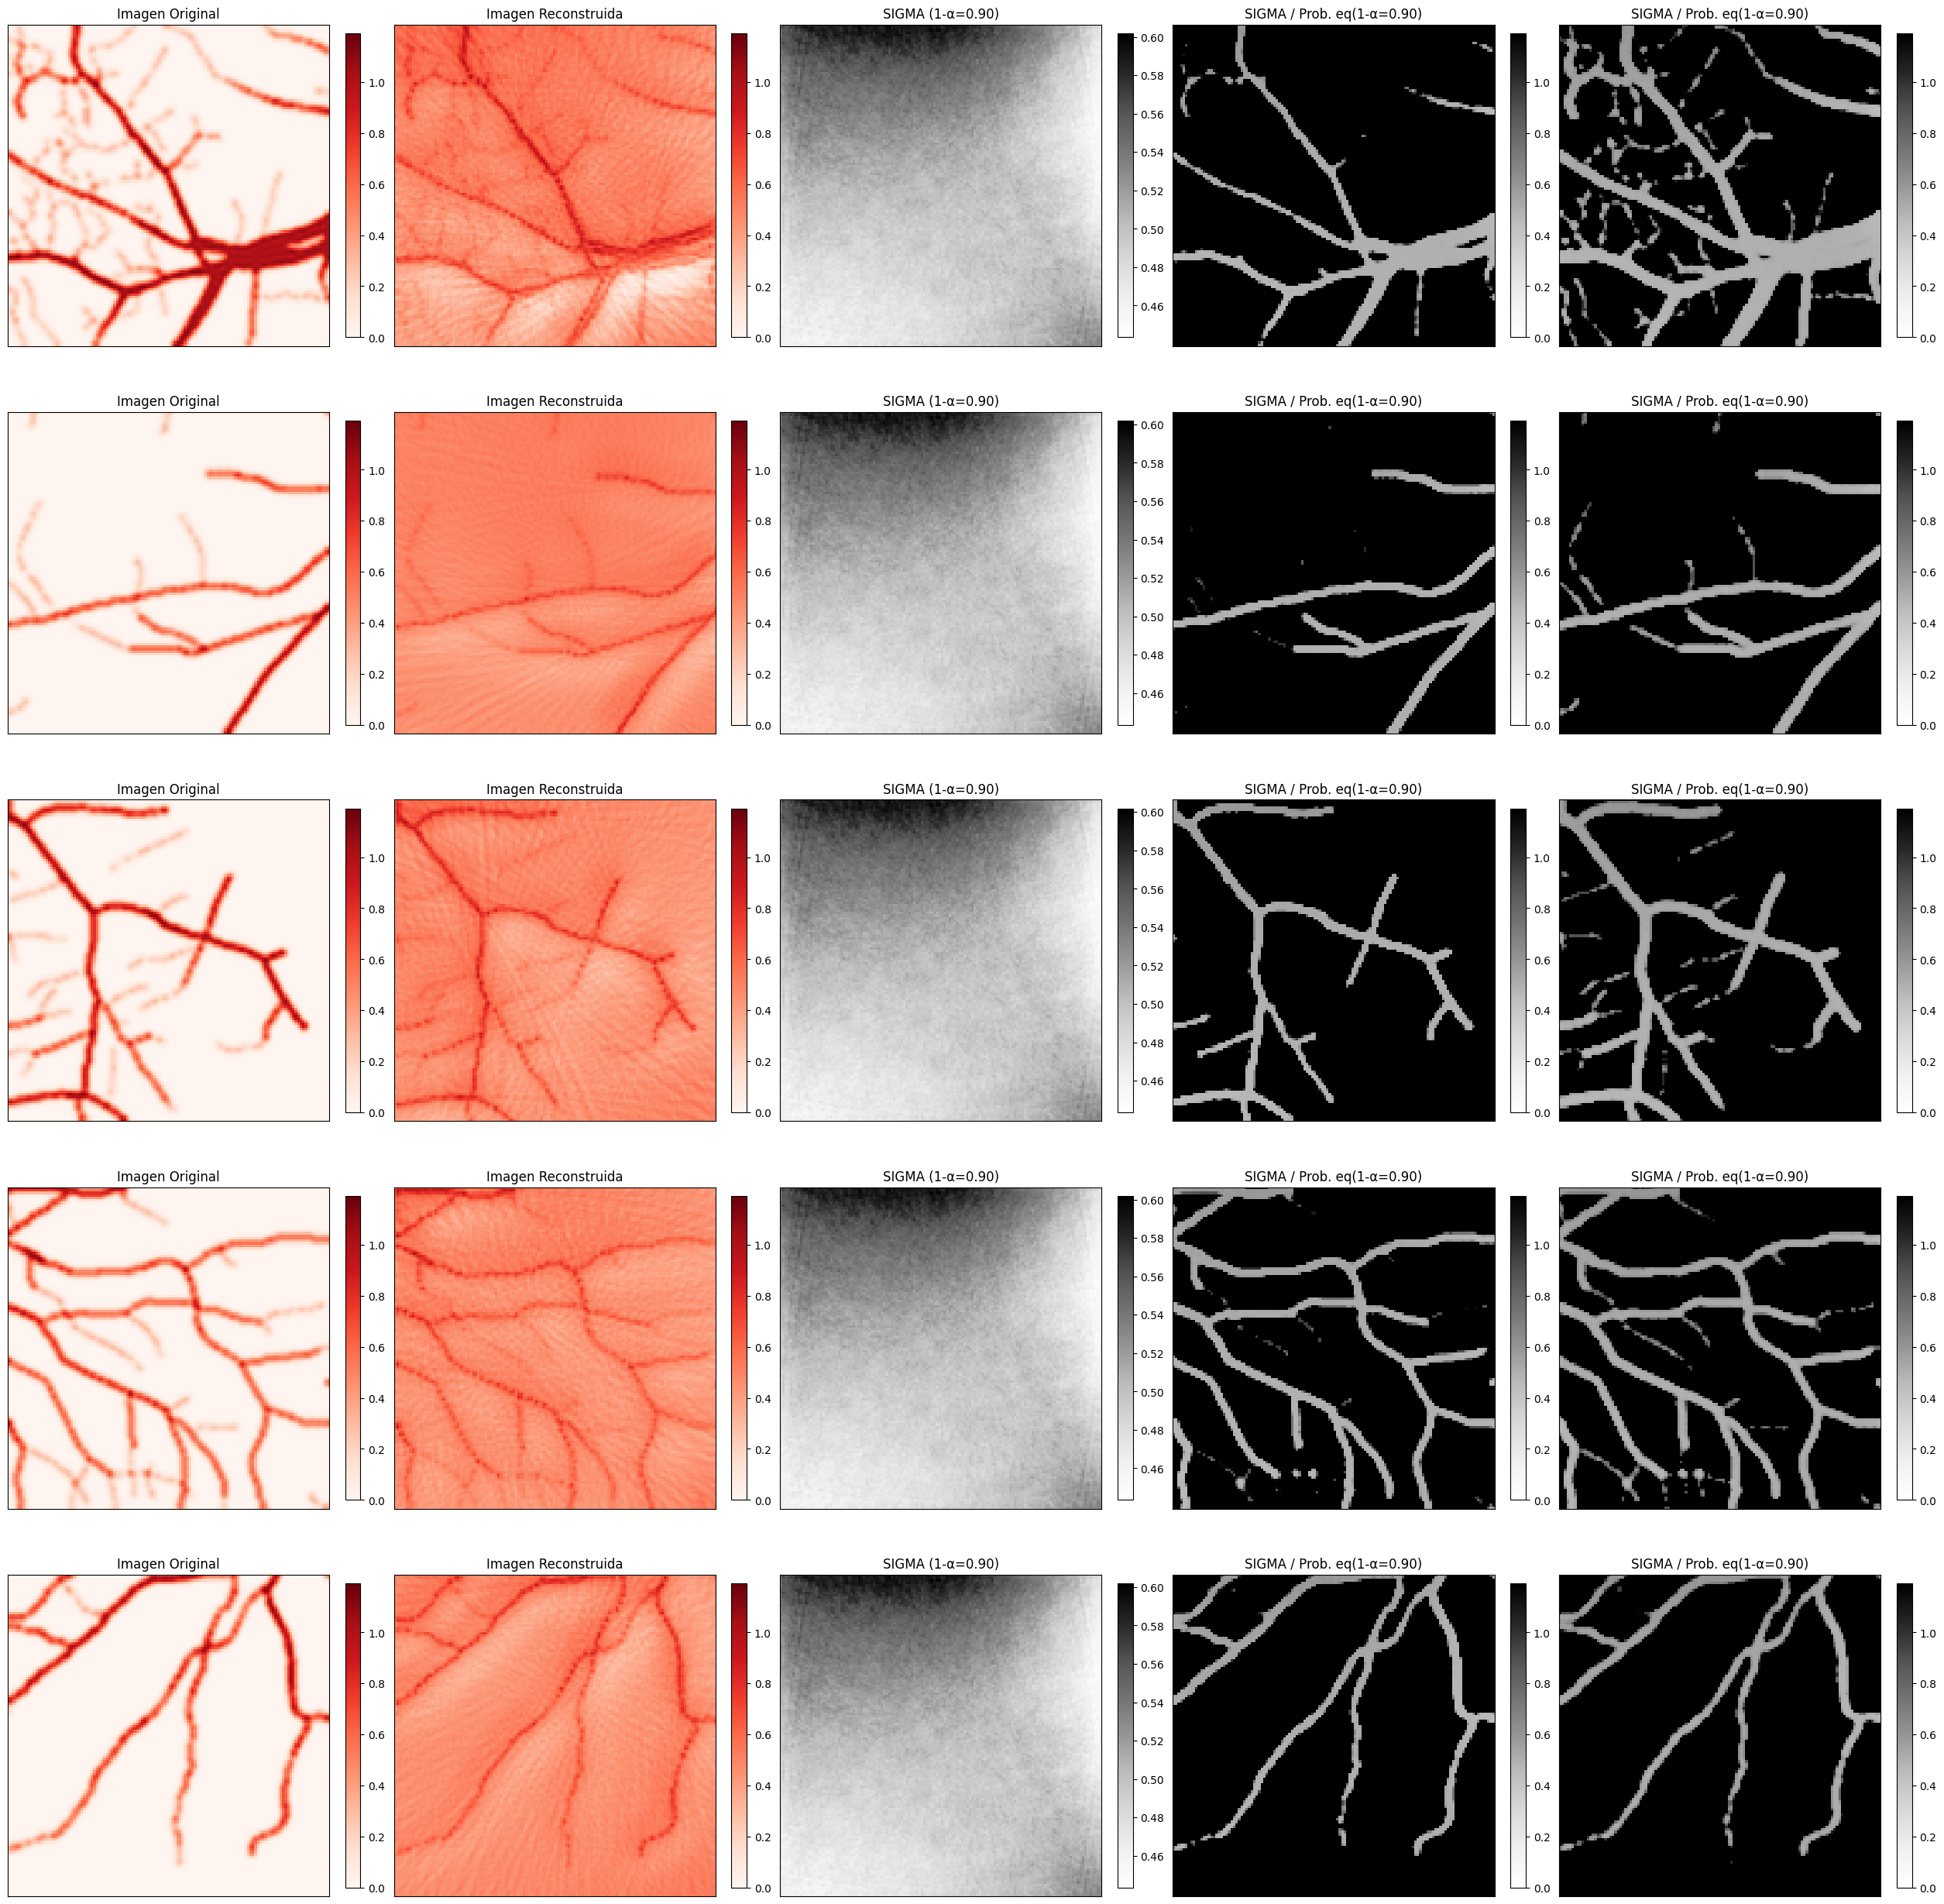
\includegraphics[width=0.75\linewidth]{img/scp_conf_EM.png}
    \caption{Split Conformal Prediction con bandas de predicción escaladas mediante la máscara de probabilidad EM.}
    \label{fig:scp_mascara}
\end{figure}

\subsubsection{SCP basado en partición binaria de clases}

A partir de la capacidad de segmentación introducida en el enfoque anterior, surge la oportunidad estratégica de fragmentar el dominio de calibración. Específicamente, se propone aplicar SCP condicional de forma aislada para el conjunto de píxeles clasificados como estructuras vasculares, y un proceso homólogo e independiente para los píxeles asignados al fondo.

Bajo este esquema, el dominio espacial se particiona en dos subconjuntos disjuntos a los cuales se les induce un proceso de calibración conforme por separado.

\begin{figure}[H]
    \centering
    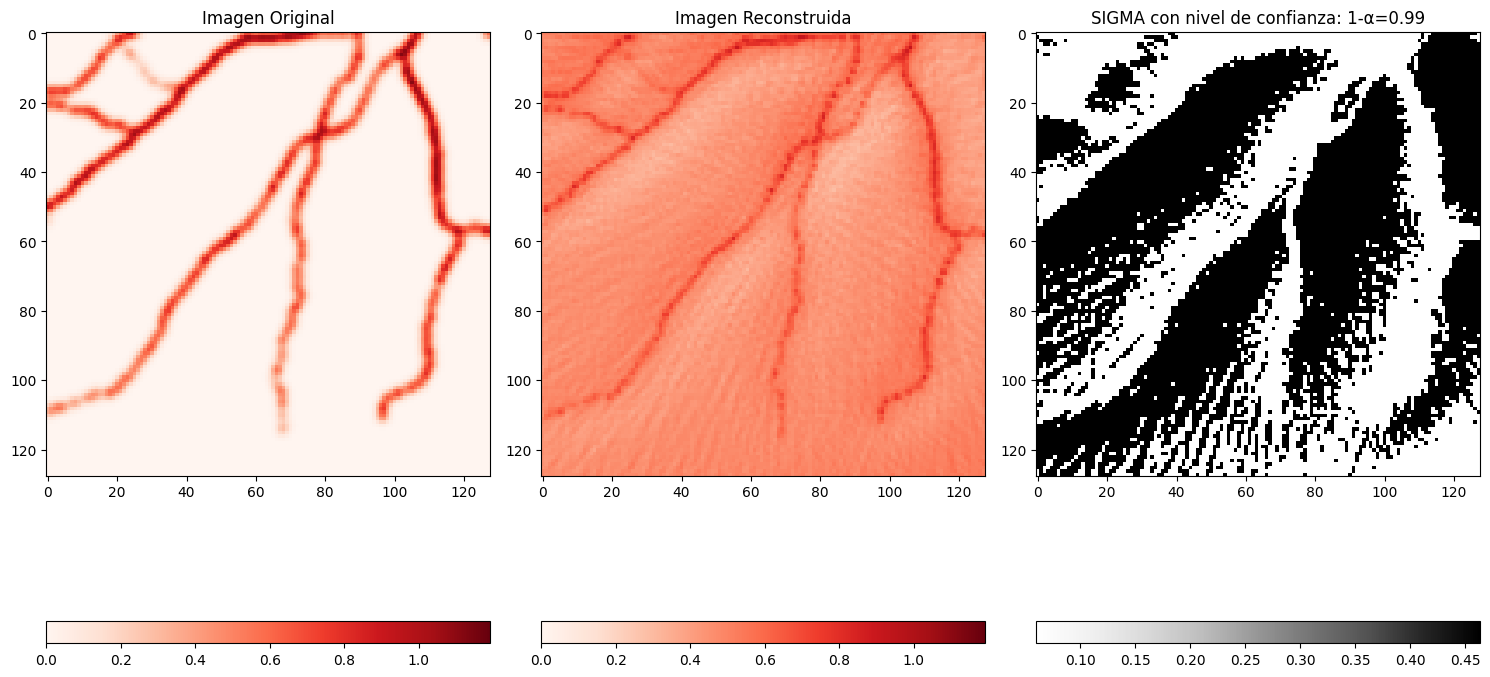
\includegraphics[width=0.75\linewidth]{img/scp_doble_em.png}
    \caption{Esquema de doble Split Conformal Prediction aplicado de forma independiente a las regiones de vena y fondo.}
    \label{fig:doble_scp_cluster}
\end{figure}

Este enfoque binario permite restringir el tamaño de los intervalos, logrando disminuir significativamente la incertidumbre en las regiones donde no se compromete la presencia de estructuras vasculares.

\subsubsection{Método de Kandinsky}

El método de Kandinsky, concebido originalmente para escenarios de clasificación, busca armonizar las ventajas de la calibración condicional local y la calibración marginal, tal como se detalla en el algoritmo~\ref{alg:kandinsky}. A través de un enfoque basado en agrupamiento espacial y pooling de puntuaciones de no conformidad, el método viabiliza estimaciones estables y estadísticamente válidas en dimensiones espaciales de alta resolución.

\begin{algorithm}[H]
    \caption{Algoritmo de Kandinsky Conformal Prediction}
    \label{alg:kandinsky}
    \begin{algorithmic}[1]
        \REQUIRE Tensor de no conformidad de calibración $\mathbf{S} \in \mathbb{R}^{N \times H \times W}$, niveles de cuantiles discretos $\mathcal{Q} = \{\tau_1, \dots, \tau_M\}$, número de clústeres $K$, nivel de significancia $\alpha$, instancia de prueba $X_{\text{test}}$.
        \ENSURE Mapa topográfico de umbrales $\mathbf{Q} \in \mathbb{R}^{H \times W}$, conjuntos de predicción válidos $\mathcal{C}_{\alpha}(X_{\text{test}})$.

        \vspace{0.1cm}
        \STATE \textbf{// Fase I: Extracción de Características Locales}
        \FOR{cada coordenada espacial $(i, j) \in \{1, \dots, H\} \times \{1, \dots, W\}$}
            \STATE Inicializar vector de perfil de riesgo: $\mathbf{x}_{i,j} \in \mathbb{R}^M$
            \FOR{$m = 1$ \TO $M$}
                \STATE $\mathbf{x}_{i,j}[m] \leftarrow \inf \left\{ q \in \mathbb{R} : \frac{1}{N} \sum_{n=1}^N \mathbb{I}(S_{n,i,j} \leq q) \geq \tau_m \right\}$
            \ENDFOR
        \ENDFOR
        \STATE Construir la matriz global de diseño: $\mathbf{X} \leftarrow \big[\mathbf{x}_{1,1}, \dots, \mathbf{x}_{H,W}\big]^T \in \mathbb{R}^{(H \cdot W) \times M}$

        \vspace{0.1cm}
        \STATE \textbf{// Fase II: Agrupamiento Espacial (Clustering)}
        \STATE Calcular la partición del dominio $\pi: \{1, \dots, H\} \times \{1, \dots, W\} \to \{1, \dots, K\}$ vía Clustering($\mathbf{X}, K$)
        \STATE Asignar la máscara estática de Kandinsky $\mathbf{M} \in \{1, \dots, K\}^{H \times W}$ tal que $\mathbf{M}_{i,j} \leftarrow \pi(i,j)$
Kandisnky2023
        \vspace{0.1cm}
        \STATE \textbf{// Fase III: Calibración Regional (Pooling)}
        \FOR{cada índice de clúster $k = 1$ \TO $K$}
            \STATE Agregar el multiconjunto de puntuaciones históricas: $\mathcal{S}_k \leftarrow \Big\{ S_{n,i,j} \;\Big|\; n \in \{1, \dots, N\}, \; \mathbf{M}_{i,j} = k \Big\}$
            \STATE Determinar el tamaño muestral efectivo regional: $N_k \leftarrow |\mathcal{S}_k| $
            \STATE Calcular el cuantil corregido: $q_k^* \leftarrow \inf \left\{ q \in \mathbb{R} : \frac{1}{N_k} \sum_{s \in \mathcal{S}_k} \mathbb{I}(s \leq q) \geq \frac{\lceil (N_k + 1)(1 - \alpha) \rceil}{N_k} \right\}$
        \ENDFOR

        \vspace{0.1cm}
        \STATE \textbf{// Fase IV: Inferencia Estática y Proyección}
        \STATE Proyectar mapa de umbrales: $\mathbf{Q}_{i,j} \leftarrow \sum_{k=1}^K q_k^* \cdot \mathbb{I}(\mathbf{M}_{i,j} = k) \quad \forall (i,j)$
        \FOR{cada píxel $(i, j) \in X_{\text{test}}$}
            \STATE $\mathcal{C}_{\alpha}(X_{\text{test}})_{i,j} \leftarrow \left\{ y \in \{1, \dots, \mathcal{Y}\} : 1 - \hat{f}(X_{\text{test}})_{i,j,y} \leq \mathbf{Q}_{i,j} \right\}$
        \ENDFOR

        \RETURN $\mathbf{Q}$, $\mathcal{C}_{\alpha}(X_{\text{test}})$
    \end{algorithmic}
\end{algorithm}

Si bien el algoritmo de Kandinsky fue concebido originalmente para problemas de clasificación, su formulación matemática permite extenderlo de manera directa al ámbito de la regresión. Dado que el método opera fundamentalmente sobre la distribución espacial de las puntuaciones de no conformidad, las funciones de score continuas provenientes de un regresor base pueden ser integradas y calibradas bajo los mismos principios de agregación regional y agrupamiento espacial descritos en las secciones anteriores.

\begin{figure}[H]
    \centering
    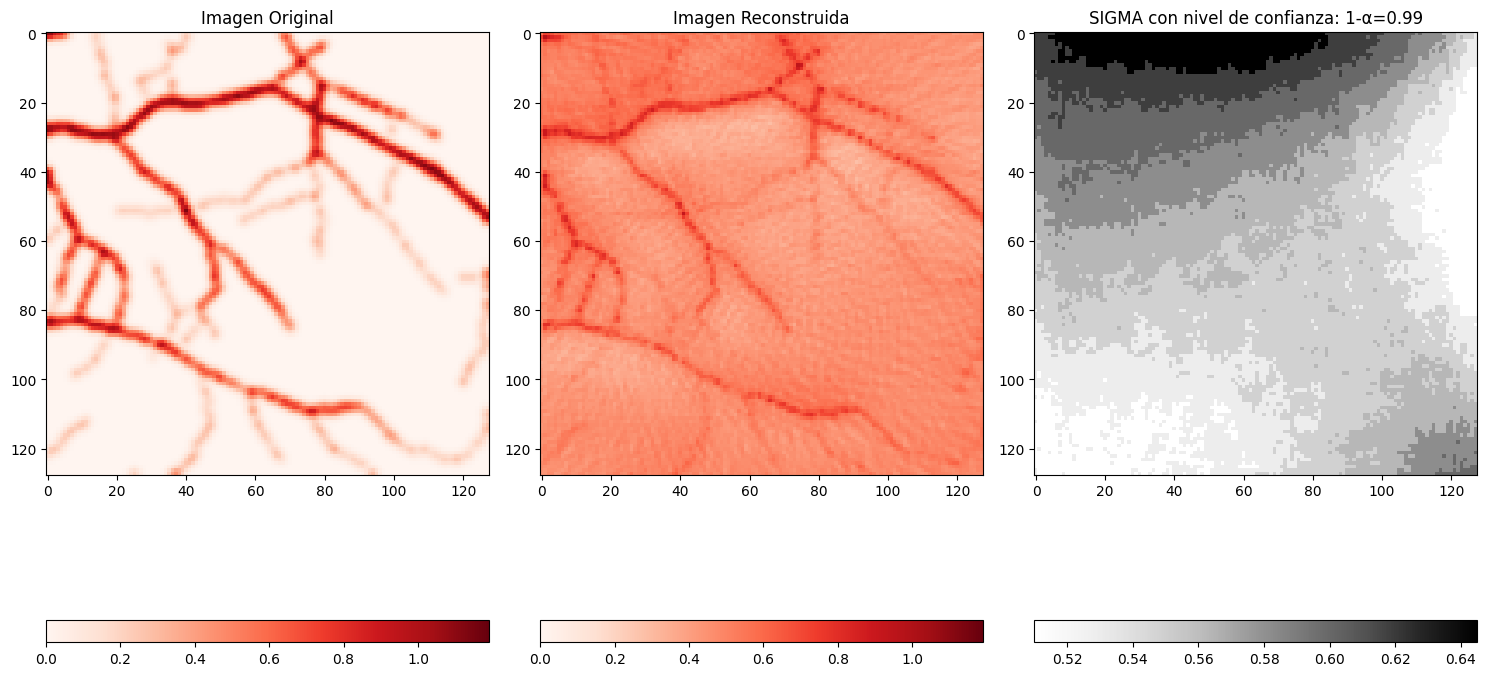
\includegraphics[width=0.75\linewidth]{img/kandinsky.png}
    \caption{Kandinsky conformal predictión}
    \label{fig:kandinsky}
\end{figure}


En la primera fase, el método condensa la información del conjunto de calibración calculando $M$ cuantiles empíricos de forma local para cada píxel. De este modo, se transforma el histórico dimensional de errores en una matriz espacial de características exógenas donde cada coordenada geométrica queda representada por un vector que describe su perfil de riesgo local.

Posteriormente, en la segunda fase, estos vectores de cuantiles actúan como las características de entrada para un algoritmo de agrupamiento parametrizado con $K$ clases, lo que permite segmentar y particionar el dominio de la imagen en una máscara estática que unifica los píxeles con dinámicas de incertidumbre estadísticamente similares.

En la tercera fase, se ejecuta un proceso de recalibración independiente sobre los componentes de cada clúster; al agregar las puntuaciones de no conformidad de todos los píxeles pertenecientes a una misma región a lo largo de todas las muestras de calibración, se produce un aumento masivo de datos que estabiliza el tamaño muestral efectivo. Este mecanismo de agregación regional no solo optimiza la precisión en la estimación del cuantil conforme global, sino que además mitiga de manera drástica el ruido heterocedástico local de alta frecuencia.

Finalmente, durante la etapa de inferencia, la predicción de cualquier instancia futura se realiza proyectando los scores del modelo sobre el mapa de umbrales estáticos e invariantes derivado de los datos aumentados, garantizando así la estabilidad y robustez de la cobertura condicional por zona.